\documentclass[a4paper]{article}

\usepackage[english]{babel}
\usepackage[utf8]{inputenc}
\usepackage{amsmath}
\usepackage{graphicx}
\usepackage[colorinlistoftodos]{todonotes}
\usepackage[utf8]{inputenc}
\usepackage[a4paper, total={6in, 8in}]{geometry}


\title{COP 290}

\author{Parichay Jindal (2013TT10937) \\ Rajat Garg (2013CH10099) \\ Silky Jain (2013TT10970) }

\date{\today}

\begin{document}
\maketitle

\section{Introduction}

This assignment involves developing a front-end as well as back-end model for registering complaints. The app shall contain following features and for each feature, we will be calling corresponding server API :
Login, view all notifications, view list of all registered complaints by user, view sorted list of resolved and unresolved complaints, post a new complaint, up-vote or down-vote the complaint(if elligible for it i.e the complaint should not be individual type and user should be one of the affected ones), change status of a complaint to resolved(if eligible) ,post a comment to a complaint, get detailed information about a particular complaint and log out.
The assignment can be further extended to web based clients by the use of well defined APIs.


\section{Data Storage}

The data will be stored in 3 tables, one table for complaints, one for users and one for notifications.\\ 
Initially the complaints and the notifications table would be empty. These would be populated along the app usage.\\
As any user logs into the app, his details would be checked against the database. The elements of a particular user in the database would include \texttt{user\char`_id}, name, \texttt{email\char`_id}, \texttt{phone\char`_no}, \texttt{user\char`_type} (owner of complaint or resolver), user-name, password etc \\
User will be now allowed to register a new complaint or update an existing complaint. On registering a new complaint, the complaint table will store the following elements related to a particular complaint in an array - 
\begin{itemize}
\renewcommand\labelitemi{--}
\item \texttt{user\char`_id}
\item User(details of user filing the complaint)
\item \texttt{Complaint\char`_id} (self-generated)
\item \texttt{Complaint\char`_type}(individual/hostel/institute level)
\item \texttt{Complaint\char`_status}
\item Date of Complaint
\item \texttt{Concerned\char`_user}
\item Description
\item Comments(array of comment details)
\item \texttt{Comment\char`_users}(array of the users who have posted the details)
\item \texttt{Upvote\char`_users}
\item \texttt{Downvote\char`_users}

\end{itemize} 

While updating an existing complaint, the server would first check the eligibility of the user from the complaint database and only the effected users will be able to up-vote and down-vote the particular complaint.\\
The \textbf{\texttt{concerned\char`_person}} will have to solve the complaint and thus the registered complaint details will be shown as notifications and also will be added to list of complaints storing the required attributes.\\
\textbf{Description} element of complaint table will store the description of that particular complaint.\\
\textbf{\texttt{Complaint\char`_status}} will help us to sort out resolved and unresolved complaints.\\
The notification table will be updated with each new complaint and comment post.\\

\section{Server APIs}
\begin{enumerate}
\item \textbf{Login} (API 1): $$/default/login.json?userid=<username>\&password=<password> $$
The server will check the username and password entered against the stored data in users table and respond.\\
Response :{"user":{(userdetails)},"success":"true"} (if correct user details else will remain the default value 'false')
\item\textbf{ Logout} (API 2): 
$$/default/logout.json$$
The cookie sessions and cache get cleared. Sets all tokens to there default values.

\item \textbf{List of all complaints} (API 3) :
$$/complaints/list.json$$
All the complaints that the logged in user has created or can view will be sorted using the user id as key, from the complaints table and added in the JSONArray complaints.\\
Response : {"complaints": [ ],"user":{details}}

\item \textbf{Resolved Complaints} (API 4) :$$ /complaints/resolvedlist.json $$
All the complaints that the logged in user has created or can view will be sorted using the user id as key, from the complaints table and added in the JSONArray resolved after checking the status of each complaint.\\
Response : {"resolved": [ ],"user":{details}}

\item \textbf{Unresolved complaints} (API 5) :$$ /complaints/unresolvedlist.json $$
All the complaints that the logged in user has created or can view will be sorted using the user id as key, from the complaints table and added in the JSONArray unresolved after checking the status of each complaint.\\
Response : {"unresolved": [ ],"user":{details}}

\item \textbf{Post a new complaint} (API 6):$$ /complaints/new.json?title=<title>\&description=<description>\& \texttt{complaint\char`_type}=<type> $$
The new complaint posted will be stored into the complaints table in the database using the user key. Also, the notifications table will be updated.\\
Response: {"\texttt{comment\char`_id}":"$<$id$>$","success":"true"} or \\
		{"\texttt{err\char`_msg}":"$<$error$>$","success":"false"} \\
Post: "notifications":"$<$name$>$ has posted a new complaint titled $<$\texttt{complaint\char`_title}$>$"

\item \textbf{Post a comment to a complaint} (API 7) :$$ /complaints/\texttt{post\char`_comment}.json?\texttt{complaint\char`_id}=<\texttt{complaint\char`_id}>\&description=<description>$$
The posted comment details will be added to the database through JSONArray comments and the user details will be added to the JSONArray \texttt{comment\char`_users}. Also, the notifications table will be updated.\\
Response:{comment:{},"user":{},"success":"true"} or\\
		{"\texttt{err\char`_msg}":"$<$error$>$","success":"false"} \\
Post: "\texttt{comment\char`_users}":"$<$userdetails$>$", "comments":"$<$comment details$>$" 

\item \textbf{Info of a particular complaint} (API 8): $$/complaints/complaint.json/<\texttt{complaint\char`_id}>$$
The \texttt{complaint\char`_id} will be used to retrieve the details of the particular comment.\\
Response:{complaint:{details},comments:[],\texttt{comment\char`_users:[]}}

\item \textbf{All notifications}(API 9) : $$/default/notifications.json$$
All the notifications corresponding to the logged in user will be retrieved.\\
Response:{"notifications":[]}

\item \textbf{Upvotes}(API 10) : $$/complaints/upvotes.json$$
The user details will be added to the JSONArray \texttt{upvote\char`_users}.\\
Response:{"user":{},"success":"true"} or\\
		{"\texttt{err\char`_msg}":"$<$error$>$","success":"false"}\\
Post: "\texttt{upvote\char`_users}":"$<$userdetails$>$"

\item \textbf{Downvote11} (API 11): $$/complaints/downvotes.json$$
The user details will be added to the JSONArray \texttt{downvotevote\char`_users}.\\
Response:{"user":{},"success":"true"} or \\
		{"\texttt{err\char`_msg}":"$<$error$>$","success":"false"} \\
Post: "\texttt{downvotevote\char`_users}":"$<$userdetails$>$"

\item \textbf{Resolve} (API 12) : $$/complaints/resolved.json$$
The status of complaint will change to resolved if the user has the power to do so.
Response:{"complaint":{},"success":"true"} or
		{"\texttt{err\char`_msg}":"$<$error$>$","success":"false"}

Except when posting a new complaint or when commenting/upvoting/downvoting a complaint, we use GET method to call the API




\end{enumerate}

\section{Flow Scheme}
\begin{figure}[ht]
\centering
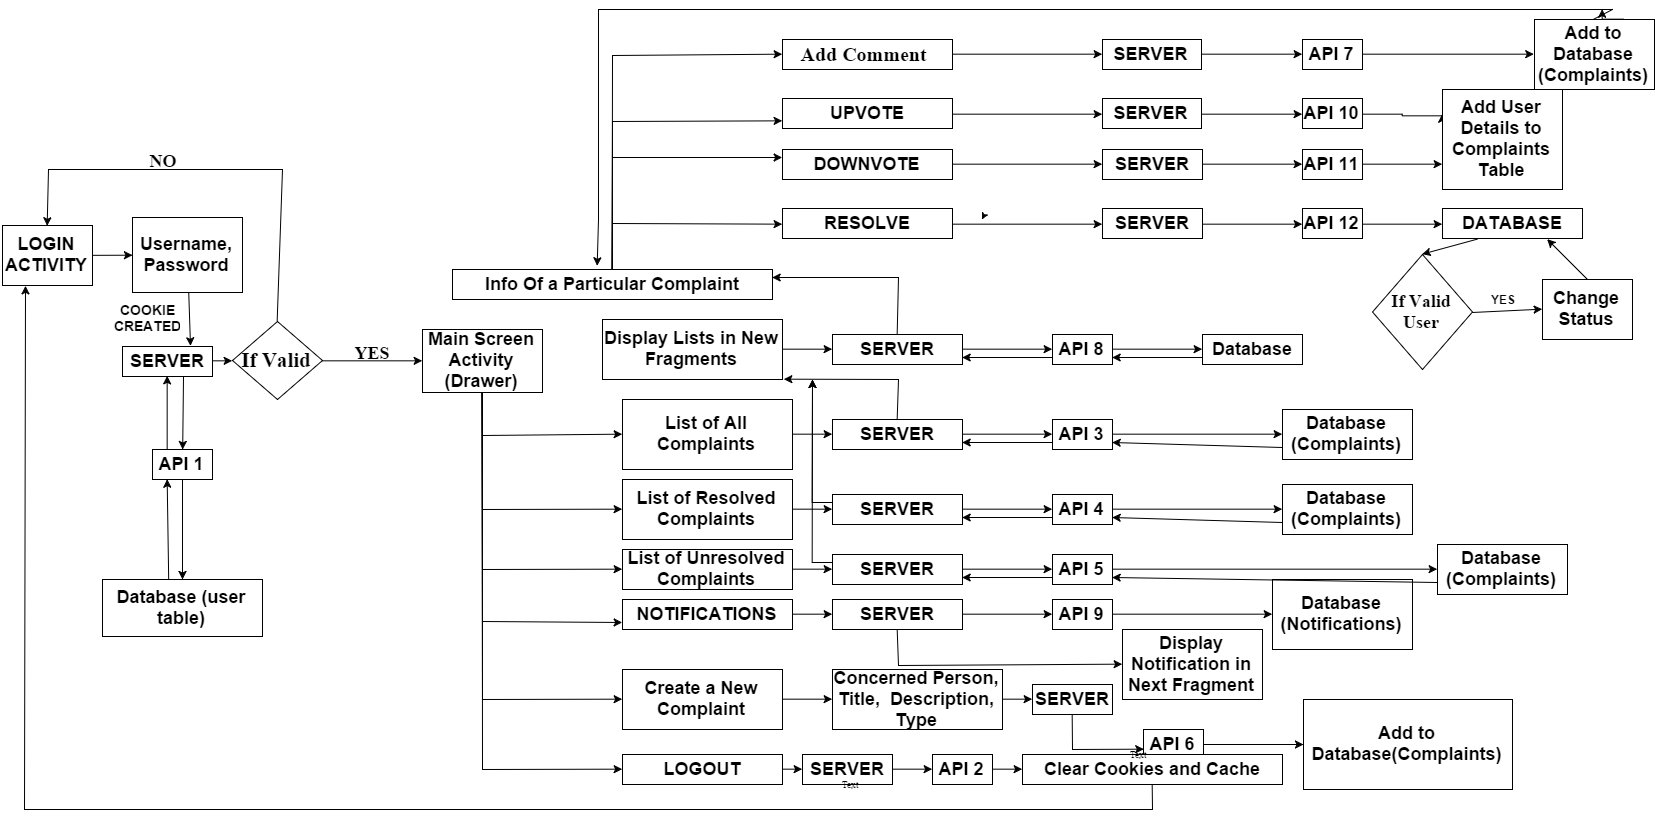
\includegraphics[width=\textwidth]{Flow.jpg}

\end{figure}

\section{BUG FORESIGHT}
\begin{enumerate}
\item Login Activity:Validation of username and password from the table users in the database.
\begin{itemize}
\item Testcase1: check for a valid username and password
\item Testcase2: check for an invalid username and password combination.
\end{itemize}
\item Main Screen Activity: Ensure correct results from each option.
\begin{itemize}
\item List of all complaints that the particular user can view/ had created should be displayed. (volley error in case of error in cookie session storage).
\item Check if the list of resolved/unresolved problems is generated after correct validation of the status of that complaint.
\item Notifications should list all notifications for that particular user.
\item Create a new complaint
\begin{itemize}
\renewcommand\labelitemi{--}
\item Testcase 1 : All fields in correct format should lead to “success”:”true”.
\item Testcase 2 : check invidually if the only valid entries are being accepted.
\item Testcase 3 : Ensure all required fields are entered before sending the data to the server.
\item Check if the complaint created can be viewed by all affected and concerned users.

\end{itemize}
\item Logout should clear all cache/cookie-sessions and check for successful login by another user.
\item Clicking on a particular complaint from the list of complaints:
\begin{itemize}
\renewcommand\labelitemi{--}
\item Information of the particular complaint should be correctly displayed.
\item Upvote/Downvote:
Check if only the \texttt{affected\char`_users} can click on this option and that only one of the options is selected. Also ensure that the user can not revote for the particular complaint.
\item Resolve:
The option should only be available for the right user.
\texttt{Concerned\char`_user} in case of individual level complaint and the user creating the complaint in case of other two types.
This option should only be used once.
Once the complaint is resolved, it should appear in the list of resolved complaint and not in unresolved complaints (status should be successfully changed in the database)
\end{itemize}
\item Add comment:
All affected and concerned users along with the user who created the complaint should be able to add comment.
\begin{itemize}
\renewcommand\labelitemi{--}
\item Testcase 1 : All fields in correct format should lead to “success”:”true”.
\item Testcase 2 : check individually if the only valid entries are being accepted.
\item Testcase 3 : Ensure all required fields are entered before sending the data to the server.
\item Check if the comment created can be viewed by all affected and concerned users along with the user who created the complaint. (The comment should be successfully stored in the complaints table along with the \texttt{comment\char`_user} information).
\end{itemize}

\end{itemize}
\end{enumerate}

\section{Moduling}
\subsection{Server Code}
We will design a Django framework using Python for this assignment. This will contain the code to store the database(Hashmaps) and link them to the different APIs.
\begin{itemize}
\item The models.py file contains a description of the database table, represented by a Python class. This class is called a model. Using it, you can create, retrieve, update and delete records in your database using simple Python code rather than writing repetitive SQL statements.
\item The views.py file contains the business logic for the page. The complaints(),users() and notifications() function are called a view.
\item The urls.py file specifies which view is called for a given URL pattern. In this case, the URL /default/complaints will call the complaints() function.
\item The notifications.html and description.html files are HTML templates that describes the design layouts to be used. It uses a template language with basic logic statement.

\end{itemize}

\subsection{Java Code}
\begin{itemize}



\item \textbf{Login Activity Class} - This will include the code for validation of user using JSON parsing from the database and will open up the next main screen only for the valid users else it will show an error dialog box. The user details will also be transferred from database to the main screen activity class. In this class we will initiate cookies.
\item \textbf{Main Screen Activity Class} - This will be a \texttt{Navigation\char`_drawer} type of activity which will include list of all activities that users can choose from according to their need. The user details will be retrieved from the previous activity. On click of a particular element the app will open up the new fragment corresponding to that choice and the required attributes will be transferred.
\item \textbf{Custom Adapter} - This class will help us to display the required list of elements directly on the screen of a particular activity and can be used in any of the activities using conventional way of implementation.
\item	\textbf{Complaints Activity Class} - This class will display list of the complaints corresponding to the user which will be in clickable form. On clicking a particular complaint, individual complaint activity screen with further details of the complaint will open up. The complaints related to the

User details will be checked using JSON parsing on the corresponding API.The required complaint details will also be transferred from database to the New complaint activity class

This class will include a validation for the complaint and will be called to check whether the complaint is resolved or unresolved by checking the status of the complaint from the corresponding API.
\item	\textbf{Particular complaint activity class} - This class will display details of the corresponding complaint which will be parsed from the complaint table using complaint details from previous activity. The details will include description of the complaint and list of all comments to that complaint. Also the user will be allowed to add an new comment, upvote/downvote and resolve(if eligible) the complaint. A customised dialog method will be included which wil take the input of new comment from the user.
\item \textbf{Notifications Activity Class} - This class will display all the notifications retrieved from the database (notifications table) through GET request.
\item \textbf{New complaint activity class} - This class will first take input from user which will include information related to the complaint like complaint type, title, description and the concerned person details. All this information will then be transferred to the server and via corresponding API calling, will be stored in the complaints table database and also the notification table database.


\end{itemize}

\section{Android Interface}
\begin{itemize}

\item The app will launch a \textbf{login activity screen} where the username and the password are requested. On click of the submit button, it will be sent to the server and validated. The user will be able to reach the next screen if valid else an error message is displayed.
\item The next \textbf{menu activity screen} will welcome the user. This will contain a drawer with a list of different options:
\begin{itemize}
\renewcommand\labelitemi{--}
\item \textbf{Create a new complaint}: On click, this will open up a new fragment where the user will be provided with four EditText boxes for entering type of complaint, reference of the concerned person to whom the complaint is made, title of the complaint and description of the complaint and a submit button to submit the complaint. A dialog box will appear incase of an error.
\item \textbf{List of all complaints}: On click, this will open a new fragment which will display the list of all the complaints created by user or affecting the user. All these complaints will be clickable.\\
On clicking a particular complaint, the decription and the comments corresponding to that complaint will be displayed in another fragment along with an option to add a new comment, upvote/downvote the complaint and resolve the complaint. Only valid users will be allowed to use these options and can either upvote or downvote the complaint only once.\\
On clicking add a new comment, a dialog box will appear where the user can enter the comment and once entered, the comment will be added to list of comments being displayed there

\item \textbf{ List of resolved complaints}: On click, this will open a new fragment which will display the list of all the complaints whose status has been changed to resolved. These are all clickable and the rest of the activities will be same as above except that there will be no option to resolve the complaint here. 

\item \textbf{List of unresolved complaints}: On click, this will open a new fragment which will display the list of all the complaints whose status is unresolved. These are all clickable and the rest of the activities will be same as when list of all complaints appear.

\item \textbf{Notifications}: The list of all notifications appear on clicking this option
\item \textbf{Logout}: This will simply return back to the login activity screen

\end{itemize}


\end{itemize}

\end{document}